\chapter{Referencial teórico}

Este capitulo apresenta os temas necessários para o desenvolvimento desse estudo e que devem ser tratados mais profundamente já que afetam o diretamente o foco principal do trabalho. Este capitulo foi estruturado em 4 tópicos, a saber: informações sobre o padrão 802.11 e as faixas utilizadas por ele, interferência de ondas, a tecnologia VLC e o projeto OpenVLC.

\section{Padrão IEEE 802.11}

Quando os computadores receberam transmissores e receptores de rádio varias empresas começaram a comercializar LANs sem fios, porém não havia uma padronização para a comunicação, ou seja, um computador equipado com um rádio da marca \emph{X} não era compatível com o computador equipado com o rádio da marca \emph{Y}. Diante deste problema surgiu a necessidade de se criar um padrão para as LANs sem fios, assim o comitê do IEEE criou o padrão 802.11 mais conhecido como \textit{wifi} \cite{tanenbaum}.

\subsection{Faixas 2.4Ghz e 5Ghz}

As faixas de radio que o \textit{wifi} utiliza são as faixas de 2,4GHz e 5GHz, as duas bandas não necessitam de licença para a sua utilização contudo os aparelhos devem limitar a sua potência para permitir que diferentes dispositivos coexistam. Como a utilização da faixa é livre é muito provável que os equipamentos de \textit{wifi} tenham que lidar constantemente com interferências \cite{tanenbaum}.

\section{Interferência de Ondas}

Se duas ondas senoidais de mesmo comprimento de onda são propagadas em uma corda no mesmo sentido mas estão defasadas, ou seja os picos estão alinhados com o vales da outra, elas se cancelam mutuamente e o deslocamento é zero. Este fenômeno chamados de interferência \cite{fisica}. 

\begin{figure}
  \caption{Demonstração das ondas resultantes}
  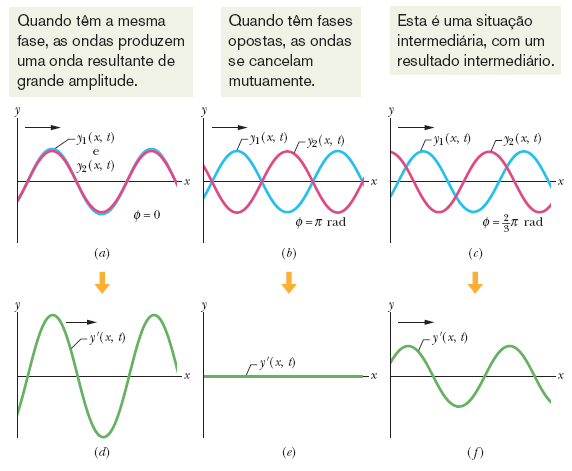
\includegraphics[width=0.6\textwidth]{images/ondas_interferencia.png}
  \legend{Fonte: \citeonline{fisica}}
  \label{fig:ondas_inter}
\end{figure}


\section{VLC}



\section{OpenVLC}

O OpenVLC é uma plataforma \textit{open source} baseada em  Linux e na plataforma Beagle Bone Black (BBB), projetada para ser de baixo custo e ser utilizada em pesquisas de redes VLC. O projeto consiste em um \textit{hardware} para a transmissão e recepção e sua implementação de \textit{software} atua na camada de enlace \cite{OpenVLCB}.

\begin{figure}[htbp]
  \begin{minipage}{0.4\textwidth}
    \caption{Diagrama do hardware do OpenVLC}
    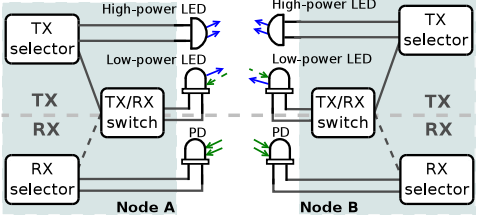
\includegraphics[scale=0.55]{images/diagram_cape_OpenVLC.png}
    \legend{Fonte: \citeonline{OpenVLCB}}
    \label{figura:diagramaVLC}
  \end{minipage}
  \hfill
  \begin{minipage}{0.4\textwidth}
    \centering
    \caption{Foto do hardware do OpenVLC} \label{fig_minipage_imagem1}
    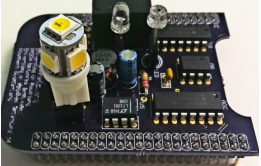
\includegraphics[scale=0.8]{images/Cape.png}
    \legend{Fonte: \citeonline{OpenVLCB}}
  \end{minipage}
\end{figure}

